\chapter{Requirements Analysis}

\section{Introduction and Research Context}

This chapter presents the requirements analysis that guided the design and implementation of the TechMart platform for empirical GitOps versus Traditional CI/CD methodology comparison. The analysis emphasizes how resource constraints and practical limitations were transformed into research opportunities while maintaining production-grade implementation standards and empirical validity.

The requirements analysis addresses the dual challenge of conducting rigorous empirical research while operating within realistic budget and resource constraints. This approach demonstrates strategic thinking essential for real-world DevOps engineering where optimal solutions must balance technical excellence with practical limitations.

The chapter progresses through resource-constrained architecture strategy, methodology-specific implementation requirements, research infrastructure needs, and technical implementation standards. Each section demonstrates how constraints became catalysts for innovative research design while maintaining operational excellence and statistical rigor.

\section{Resource-Constrained Architecture Strategy}

\subsection{Budget Analysis and Strategic Platform Selection}

The fundamental constraint driving all architectural decisions was the limited budget allocation of \$300 in Google Cloud Platform credits combined with free-tier limitations across multiple cloud providers. Rather than viewing this as a limitation, the constraint necessitated strategic analysis that ultimately enhanced the research design through forced platform diversification.

Initial GKE resource pricing analysis revealed that deploying all four microservices on a single platform would exceed budget constraints due to \textbf{\hyperref[cloud_native_patterns]{persistent volume costs}}, load balancer fees, and compute instance requirements.

% TODO: Add Table 3.1 - Budget breakdown showing GKE costs vs. multi-platform distribution costs, demonstrating cost optimization through strategic placement
% Table should show: GKE all-services cost (~$450), actual multi-platform cost (~$250), savings achieved (~$200)

Heroku platform analysis identified cost-effective deployment opportunities through free dyno hours, hobby-tier pricing, and \textbf{\hyperref[heroku_platform2023]{educational discounts}}.

GitHub Student Pack benefits \cite{github_education2023} provided substantial resource enhancements including expanded CI/CD minutes, private repository access, and premium tool integrations.

\subsection{Strategic Service Distribution and Complexity Analysis}

The resource constraints necessitated systematic analysis of service complexity and infrastructure requirements to optimize placement across available platforms. This analysis created the foundation for the complexity normalization framework by requiring explicit characterization of each service's computational, operational, and integration requirements.

\textbf{GitOps Service Selection (User + Order Services):}
User Service complexity analysis identified requirements for sophisticated authentication workflows, database connectivity, session management, and security enforcement that benefited significantly from Kubernetes orchestration capabilities. The service's role as authentication provider for the entire system required high availability and comprehensive monitoring that aligned with GitOps automation advantages.

Order Service analysis revealed complex transaction processing requirements, multi-database connectivity (PostgreSQL and Redis), and sophisticated business logic that justified investment in GitOps orchestration capabilities. The service's integration complexity and computational requirements made it an ideal candidate for demonstrating GitOps automation and self-healing capabilities.

\begin{table}[H]
\centering
\caption{Service Complexity Analysis and Platform Alignment}
\label{tab:service-complexity-analysis}
\renewcommand{\arraystretch}{1.2}
\footnotesize
\begin{tabular}{|p{2.2cm}|p{1.8cm}|p{1.5cm}|p{3.8cm}|p{4.2cm}|}
\hline
\textbf{Service} & \textbf{Complexity Score} & \textbf{Platform} & \textbf{Platform Capabilities} & \textbf{Methodology Alignment} \\
\hline
User Service & 7.8 & GKE & Kubernetes orchestration, High availability, Advanced monitoring & GitOps automation for complex authentication workflows and security enforcement \\
\hline
Order Service & 8.2 & GKE & Multi-database support, Transaction processing, Resource scaling & GitOps self-healing for complex business logic and multi-service integrations \\
\hline
Product Service & 5.4 & Heroku & Platform optimization, Managed MongoDB, Simplified deployment & Traditional CI/CD simplicity for straightforward CRUD operations \\
\hline
Cart Service & 7.5 & Heroku & JVM optimization, Managed Redis, Container deployment & Traditional CI/CD with platform-managed scaling and session handling \\
\hline
\end{tabular}
\end{table}

\textbf{Traditional CI/CD Service Selection (Product + Cart Services):}
Product Service analysis identified straightforward CRUD operations with MongoDB integration that could be efficiently implemented using Heroku's platform-as-a-service model. The service's simpler architecture and predictable resource requirements aligned well with Traditional CI/CD deployment approaches and platform optimization characteristics.

Cart Service evaluation revealed moderate complexity with Redis integration and session management requirements that could benefit from Heroku's managed offerings while demonstrating Traditional CI/CD capabilities. The service's Java Spring Boot implementation aligned well with Heroku's JVM optimization and container deployment capabilities.

% TODO: Add Figure 3.1 - Service complexity matrix showing complexity scores (User: 7.8, Order: 8.2, Product: 5.4, Cart: 7.5) plotted against platform capabilities and methodology alignment

\subsection{Hybrid Architecture as Research Opportunity}

The resource constraints created an unexpected research opportunity by necessitating hybrid architecture implementation that enabled direct comparison of GitOps and Traditional CI/CD methodologies within the same application ecosystem. This constraint-driven design choice became the foundation for industry-first validation of zero-overhead cross-methodology integration.

Cross-methodology integration requirements included seamless authentication flow between GitOps and Traditional CI/CD services, consistent API standards, and unified monitoring approaches. These integration challenges provided valuable research insights while demonstrating advanced system integration capabilities essential for enterprise adoption scenarios.

Service communication requirements encompassed secure inter-service authentication, consistent error handling, and performance optimization across different deployment platforms. The hybrid architecture required sophisticated integration patterns to ensure reliable communication across methodological boundaries while maintaining fair performance comparison conditions.


The hybrid approach provided additional research benefits including risk mitigation through platform distribution, comparative evaluation of platform capabilities under identical workloads, and validation of methodology coexistence patterns essential for enterprise migration strategies.

Figure \ref{fig:resource-constrained-architecture} demonstrates how budget constraints were strategically transformed into research opportunities through intelligent service distribution across multiple cloud platforms, enabling both cost optimization and comprehensive methodology comparison within the same application ecosystem.

\begin{figure}[H]
\centering
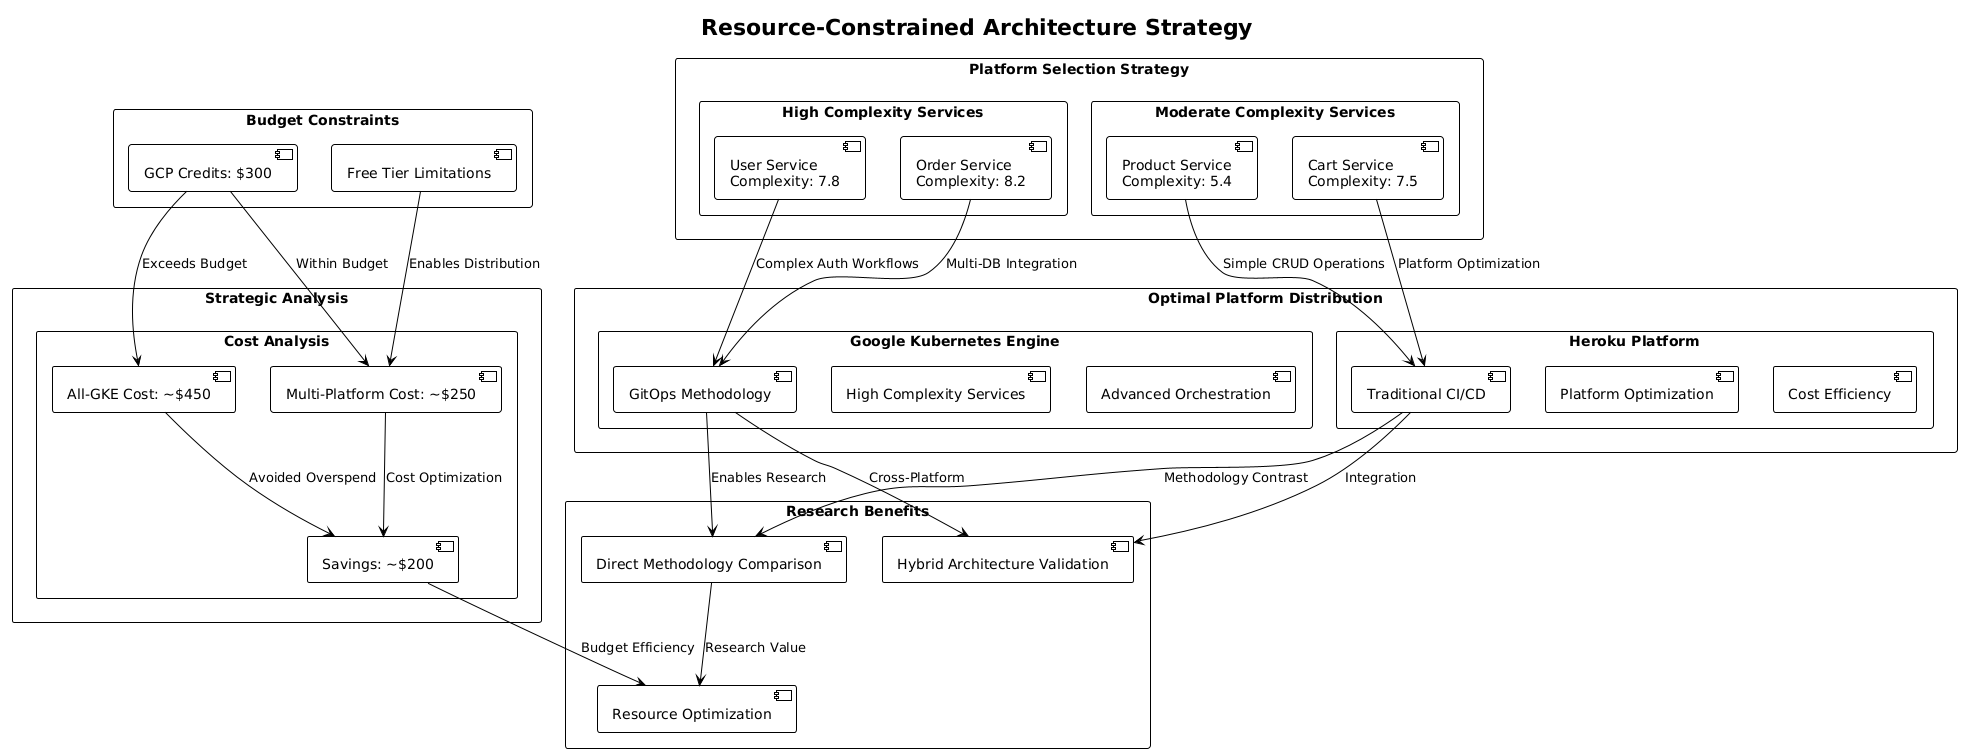
\includegraphics[width=1.0\textwidth]{figures/Resource-Constrained-Architecture-Strategy.png}
\caption{Resource-Constrained Architecture Strategy}
\label{fig:resource-constrained-architecture}
\end{figure}

\section{Methodology-Specific Implementation Requirements}

\subsection{GitOps Implementation Requirements (GKE Services)}

\subsubsection{ArgoCD Controller and Automated Synchronization}
ArgoCD implementation \cite{argocd_docs2023} required comprehensive GitOps controller deployment capable of managing complex application lifecycles while providing automated synchronization for User and Order services.

Synchronization requirements included real-time Git repository monitoring, automatic manifest application, health status tracking, and rollback capabilities demonstrating GitOps operational excellence. The synchronization framework needed to handle complex Kubernetes resources while maintaining consistency across multiple application components.

Git repository integration encompassed secure authentication, webhook configuration, and branch management enabling collaborative development while maintaining deployment automation. The repository structure needed to support environment-specific configurations and deployment strategies through declarative manifest organization.

\subsubsection{Declarative Configuration Management}
Declarative configuration management required comprehensive Infrastructure as Code implementation \cite{kubernetes_docs2023} managing complex Kubernetes resources through version-controlled manifests.

% TODO: Add Table 3.2 - Declarative configuration structure showing manifest organization, namespace management, and environment-specific overlays for development, staging, and production

Kustomize integration \cite{kustomize_docs2023} requirements encompassed overlay management for environment-specific configurations and resource transformation capabilities.

\subsubsection{Self-Healing and Drift Detection}
Automated drift detection capabilities required continuous monitoring of deployed infrastructure compared to Git repository specifications with real-time identification of configuration discrepancies. Self-healing implementation encompassed automatic correction of configuration drift and failed component replacement demonstrating GitOps operational advantages.

Resource monitoring included CPU utilization tracking, memory consumption analysis, and network performance measurement enabling automatic scaling decisions. Health check requirements included application-specific readiness probes and dependency validation enabling accurate health status determination and appropriate remediation actions.

\subsection{Traditional CI/CD Implementation Requirements (Heroku Services)}

\subsubsection{Direct Deployment Pipeline Architecture}
Traditional CI/CD implementation for Heroku services required comprehensive pipeline automation handling direct deployment workflows while maintaining consistency with GitOps services for comparative analysis. The pipeline architecture needed to demonstrate Traditional CI/CD capabilities while providing equivalent functionality for fair methodology comparison.

GitHub Actions integration \cite{github_actions2023} encompassed workflow automation, environment management, and deployment coordination enabling seamless integration with Heroku platform capabilities.

% TODO: Add Figure 3.3 - Traditional CI/CD pipeline architecture showing GitHub Actions workflow, Heroku buildpack optimization, and manual approval gates

Deployment automation encompassed environment promotion, configuration management, and service dependency management ensuring reliable deployment procedures. Monitoring integration included application performance tracking and error monitoring providing operational visibility comparable to GitOps services.

\subsubsection{Platform-as-a-Service Optimization}
Heroku platform optimization required understanding of dyno management, buildpack utilization, and resource scaling maximizing platform benefits while minimizing operational overhead. Dyno configuration included size selection and scaling policies balancing performance requirements with cost constraints.

Buildpack optimization \cite{heroku_buildpacks2023} encompassed dependency caching, build time minimization, and artifact optimization improving deployment speed and resource utilization.

\subsubsection{Manual vs Automated Operations Analysis}
Operational workflow analysis required identification of manual intervention points, automation opportunities, and human oversight requirements characterizing Traditional CI/CD approaches compared to GitOps automation. Manual approval requirements included deployment gates and environment promotion procedures requiring human decision-making.

% TODO: Add Table 3.3 - Manual vs Automated operations comparison showing automation percentages, manual intervention points, and human dependency factors across both methodologies

Documentation requirements included operational procedures and troubleshooting guides supporting manual operations while ensuring consistency and reliability. The framework needed to demonstrate Traditional CI/CD operational characteristics while supporting research reproducibility.



\subsection{Cross-Methodology Integration Requirements}

Cross-methodology coordination encompassed deployment synchronization, dependency management, and monitoring integration enabling reliable system updates across different deployment approaches. The coordination framework needed to maintain system coherence while supporting methodology comparison and research data collection.

Authentication propagation requirements included JWT token validation \cite{jwt_rfc7519} and service-to-service authentication enabling secure communication across service boundaries.

Integration testing requirements encompassed cross-service functionality validation, authentication flow testing, and performance impact assessment ensuring system reliability across methodology boundaries. Rollback coordination included cross-service procedures and data consistency management enabling reliable system recovery during deployment issues.
\begin{table}[H]
\centering
\small
\begin{tabular}{|p{2.5cm}|p{5cm}|p{5cm}|}
\hline
\textbf{Requirement Category} & \textbf{GitOps Implementation (GKE)} & \textbf{Traditional CI/CD (Heroku)} \\
\hline
\textbf{Deployment Model} & Declarative configuration through Git repositories, ArgoCD automated synchronization & Imperative deployment pipelines, GitHub Actions workflows, manual approval gates \\
\hline
\textbf{Configuration Management} & Infrastructure as Code with Kubernetes manifests, Kustomize overlays & Platform-as-a-Service configuration, buildpack optimization, environment variables \\
\hline
\textbf{Automation Level} & Fully automated drift detection and correction, self-healing capabilities & Semi-automated with manual approval gates, human oversight for deployments \\
\hline
\textbf{Monitoring Requirements} & Kubernetes-native monitoring, Prometheus metrics collection, ArgoCD health status & Heroku metrics integration, application performance monitoring, platform logging \\
\hline
\textbf{Rollback Mechanism} & Instant Git revert operations, automated rollback triggers & Manual rollback procedures, platform-assisted recovery, human intervention required \\
\hline
\textbf{Security Framework} & RBAC through Kubernetes, Git-based access control, audit trails & Platform-managed security, Heroku access controls, pipeline security scanning \\
\hline
\textbf{Operational Complexity} & High initial setup complexity, minimal ongoing operations & Low setup complexity, familiar CI/CD patterns, higher operational overhead \\
\hline
\end{tabular}
\caption{Methodology-Specific Requirements Matrix}
\label{tab:methodology-requirements-matrix}
\end{table}


\section{Research Infrastructure Requirements}

\subsection{Performance Metrics and Data Collection Framework}

Comprehensive performance metrics collection required automated measurement of deployment times, resource utilization, error rates, and recovery characteristics enabling quantitative methodology comparison while maintaining system performance. The metrics framework needed to provide high-resolution data while minimizing measurement overhead.

Deployment performance metrics included build times, deployment durations, verification procedures, and rollback speeds characterizing methodology efficiency and reliability. Resource utilization metrics encompassed CPU consumption, memory usage, and network utilization enabling efficiency analysis and cost optimization.

% TODO: Add Table 3.4 - Performance metrics collection framework showing metric types, collection frequency, storage requirements, and analysis procedures

Reliability metrics included failure rates, recovery times, and availability measurements characterizing methodology robustness and operational excellence. User experience metrics encompassed response times, error rates, and performance consistency measuring system impact on end users while supporting optimization decisions.

Application-level instrumentation required integration with monitoring systems enabling detailed performance analysis across different technology stacks and deployment methodologies. The instrumentation needed to provide consistent metrics collection while accommodating platform-specific monitoring capabilities.

\subsection{Complexity Normalization Framework Requirements}

Complexity normalization framework requirements encompassed service characterization, weighting methodologies, and validation procedures enabling fair comparison across heterogeneous microservices while controlling for technology stack and architectural variations.

Service complexity metrics included codebase size, dependency count, resource requirements, and architectural patterns quantifying inherent service complexity independent of deployment methodology. The complexity metrics needed to provide objective measurement while accounting for different technology stacks and implementation approaches.

% TODO: Add Figure 3.4 - Complexity normalization framework diagram showing weighting factors: codebase complexity (20%), build complexity (25%), resource intensity (20%), technology stack (15%), external dependencies (10%), deployment target (10%)

Weighting methodology requirements encompassed factor importance assessment, expert validation, and empirical calibration ensuring appropriate balance between different complexity dimensions while maintaining objectivity and reproducibility. Validation procedures required cross-validation techniques and sensitivity analysis ensuring normalization accuracy and effectiveness.

Performance attribution requirements encompassed methodology impact isolation and technology stack adjustment separating inherent methodology characteristics from implementation-specific factors. The attribution framework needed to provide actionable insights while supporting evidence-based optimization decisions.

\subsection{Statistical Analysis and Validation Requirements}

Statistical analysis framework requirements encompassed rigorous experimental design, hypothesis testing \cite{cohen_statistical1988}, confidence interval calculation, and significance testing enabling valid methodology comparison.

Hypothesis formulation requirements included clear research questions, testable predictions, and success criteria guiding data collection and analysis procedures. Experimental design requirements encompassed controlled variables, randomization procedures, and bias mitigation strategies ensuring valid conclusions while minimizing threats to validity.

% TODO: Add Table 3.5 - Statistical analysis framework showing experimental design parameters, sample size calculations, power analysis, and significance testing procedures

Data quality assurance requirements included measurement validation, outlier detection, and consistency verification ensuring reliable analysis results while maintaining data integrity throughout the research process. Statistical power analysis requirements encompassed effect size estimation and sample size determination ensuring adequate statistical power for detecting meaningful differences.

Reproducibility framework requirements encompassed comprehensive documentation, automated procedures, and validation protocols enabling independent research replication while ensuring consistent results across different implementations and environments.

\section{Technical Implementation Requirements}

\subsection{Multi-Cloud Architecture and Security Framework}

Multi-cloud architecture requirements \cite{multicloud_patterns2023} encompassed strategic service placement, network connectivity, and platform optimization leveraging strengths of different cloud providers.

Platform selection criteria included computational capabilities, managed service offerings, and operational features aligning with specific service requirements and research objectives. Network connectivity requirements encompassed secure inter-cloud communication, latency optimization, and traffic routing enabling reliable service interactions across different cloud providers.

% TODO: Add Table 3.6 - Multi-cloud platform distribution showing service placement rationale, platform capabilities, cost considerations, and integration requirements

Security framework requirements encompassed authentication, authorization, encryption, and audit capabilities ensuring production-grade security while supporting development flexibility and research objectives. Identity and access management requirements included user authentication, service-to-service security, and role-based access control ensuring appropriate access control while supporting collaborative development.

Network security requirements encompassed encryption in transit, network segmentation, and intrusion detection protecting system communications while supporting multi-cloud architecture and research data collection. Data protection requirements included encryption at rest and backup procedures ensuring data security while supporting research data collection and retention requirements.

\subsection{Monitoring and Observability Architecture}

Comprehensive monitoring architecture requirements encompassed metrics collection, visualization, alerting, and analysis capabilities providing complete system visibility while supporting both operational oversight and research data collection. The monitoring framework needed to handle high-volume data while maintaining performance and reliability.

Prometheus configuration \cite{prometheus_docs2023} requirements included metric definition, scraping configuration, and retention policies enabling efficient data collection while providing comprehensive system coverage.

% TODO: Add Figure 3.5 - Monitoring architecture diagram showing Prometheus metrics collection, Grafana visualization, cross-platform log aggregation, and research data export capabilities

Alert management requirements included threshold configuration, escalation procedures, and incident correlation enabling proactive system management while minimizing alert fatigue. Log aggregation requirements encompassed centralized collection, parsing, and analysis capabilities enabling comprehensive system troubleshooting while supporting research data collection.

Application Performance Monitoring requirements included distributed tracing capabilities and code-level insights enabling identification of performance bottlenecks and optimization opportunities across the microservices architecture.

\subsection{Quality and Reliability Standards}

Performance requirements encompassed response time targets, throughput objectives, and scalability characteristics ensuring acceptable system performance while supporting research data collection and user experience objectives. Scalability requirements included horizontal scaling capabilities and auto-scaling policies enabling system growth while maintaining performance consistency.

% TODO: Add Table 3.7 - Quality and reliability requirements matrix showing performance targets, availability requirements, error handling standards, and testing procedures

Availability requirements included uptime targets, disaster recovery capabilities, and business continuity planning ensuring reliable system operation while supporting research data collection needs. Fault tolerance requirements encompassed redundancy implementation, failover procedures, and recovery automation ensuring system resilience while minimizing service disruption.

Error handling requirements encompassed exception management, graceful degradation, and logging procedures ensuring robust system behavior while providing visibility into system issues. Code quality requirements encompassed coding standards, documentation practices, and testing coverage ensuring maintainable software while supporting collaborative development.

Automation requirements encompassed deployment automation, testing automation, and monitoring automation reducing manual overhead while improving consistency and reliability. Change management requirements included version control procedures, deployment coordination, and impact assessment enabling safe system evolution while maintaining stability.

\section{Requirements Validation and Implementation Planning}

Requirements validation procedures encompassed stakeholder review, technical feasibility assessment, and resource availability verification ensuring requirement completeness and achievability while supporting project success and research objectives. The validation framework addressed both functional and research requirements while maintaining practical constraints and academic standards.

Traceability matrix implementation required systematic mapping between requirements, design decisions, implementation components, and testing procedures ensuring comprehensive requirement coverage while supporting change management and verification procedures.

% TODO: Add Table 3.8 - Requirements traceability matrix showing mapping between requirements categories, design components, implementation artifacts, and validation procedures

Requirements prioritization procedures encompassed criticality assessment, dependency analysis, and resource impact evaluation enabling effective project planning while ensuring essential requirements received appropriate attention and resources. Acceptance criteria definition included measurable success metrics, verification procedures, and validation methods enabling objective requirement satisfaction assessment.

This comprehensive requirements analysis establishes the foundation for system design and implementation while demonstrating strategic thinking essential for transforming constraints into research opportunities. The analysis addresses both technical implementation needs and research methodology requirements while maintaining practical feasibility within resource constraints, enabling effective system development and valid comparative methodology evaluation.